\documentclass[article,A4,12pt]{llncs}
\usepackage[T1]{fontenc}
\usepackage{amsmath}
\usepackage{amssymb}
\usepackage{amsfonts}
\usepackage{mathrsfs, bm}

\usepackage{graphicx}
\usepackage{tabularx}
\usepackage{subfig}
\usepackage{epsf,times}
\usepackage{color}
\usepackage{wrapfig}
\usepackage{cases}
\usepackage{multicol}

\usepackage[T1]{fontenc}
%\newcommand{\tmname}[1]{\textsc{#1}}
%\newcommand{\tmop}[1]{\ensuremath{\operatorname{#1}}}
%\newcommand{\tmsamp}[1]{\textsf{#1}}
%\newcommand{\tmtextsc}[1]{{\scshape{#1}}}
%\newcommand{\tmtextsl}[1]{{\slshape{#1}}}
%\newcommand{\tmtexttt}[1]{{\ttfamily{#1}}}

\leftmargin=0.0cm
\oddsidemargin=0.5cm
\evensidemargin=0.5cm
\topmargin=0cm
\textwidth=16.0cm
%\textheight=21.5cm
\textheight=20.0cm
\pagestyle{plain}
\setlength{\columnsep}{20pt}

\def\m{\mathbf{m}}
\def\H{\mathbf{H}}
\def\E{\mathbf{E}}
\newcommand{\vepsi}{{\varepsilon}}
\def\hnorm#1#2{\vert\,#1\,\vert_{#2}}
\newcommand{\R}{{\mathbb R}}
\newcommand{\Sph}{{\mathbb S}}
\def\x{\mathbf{x}}
\def\hvec{\overline{\mathbf{h}}}
\def\evec{\overline{\mathbf{e}}}

\newcommand{ \etal}{\mbox{\emph{et al. }}}

\newcommand\vect[1]{\mbf{#1}}
\newcommand{\mbf}[1]{\mbox{\boldmath$#1$}} 
\newcommand{\RC}[1]{#1 $\times$ #1 $\times$ #1}
\def\um{$\mu$m}
\def\C{$^{\circ}\mathrm{C}$}

\newcommand{\Rmnum}[1]{\expandafter\@slowromancap\romannumeral #1@}

% DEFINITION OF CUSTOM FONT SIZE
\newcommand{\customfontA}{\fontsize{50}{55}\selectfont}
\newcommand{\customfontB}{\fontsize{14.4}{20}\selectfont}
\newcommand{\customfontC}{\fontsize{30}{35}\selectfont}

\DeclareMathAlphabet{\mathpzc}{OT1}{pzc}{m}{it}

\def\clovek#1{\noindent\bgroup\vbox{\noindent#1}\egroup\vskip1em}

% TO INPUT BACKGROUND IMAGE
\usepackage{eso-pic}
\newcommand\BackgroundPic{
\put(0,0){
\parbox[b][\paperheight]{\paperwidth}{
\vfill
\centering

\includegraphics[width=\paperwidth,height=\paperheight]{img/intro-frontpage.png}
%\includegraphics[width=\paperwidth,height=\paperheight]{img/background.jpg}
\vfill
}}}

\begin{document}

% INPUTTING BACKGROUND IMAGE
\AddToShipoutPicture{\BackgroundPic}
\vbox{}
\pagestyle{empty}
\newpage
\textwidth=15.5cm
\ClearShipoutPicture
\newpage

%%%%%%%%%%%%%%%%%%%%%%%%%%%%%%%%%%%%%%%%%%%%%%%%%%%%%%%%%%%%%%%%%%%%%%%%%

\section*{}
\small
\subsection*{About NCLab}
Networked Computing Laboratory (NCLab) is a popular Internet-based framework for 
programming, mathematics, computer modeling, 
and scientific computing. It serves students, instructors, researchers, and the general 
public. NCLab can be used free of charge for personal non-commercial purposes such as 
private hobby or self-education, as well as for individual non-funded academic research.
All other use is subject to {\bf purchasing a license} for a symbolic fee. The fees are as low as 
\$1 per user per month for educational use, and they are used to support the development 
and operational expenses. NCLab is a product of FEMhub Inc. The name "NCLab" is 
registered with the U.S. Patent and Trademark Office (USPTO) under Trademark No. 85420518.

\subsection*{Terms of Use and Pricing}
More details on purchasing a license and using NCLab are provided in the online documents 
{\bf Pricing} and {\bf Terms of Use} that are accessible from NCLab's home page 
{\tt http://nclab.com}.

\subsection*{Contact Information}
General inquiries: {\tt info@femhub.com}\\
Sales: {\tt sales@femhub.com}\\
NCLab support: {\tt support@nclab.com}\\
Agros \& Hermes support: {\tt support@femhub.com}\\
Web page: {\tt http://femhub.com}\\
{Physical address}\\
FEMhub Inc.\\
5490 Twin Creeks Dr.\\
Reno, NV 89523

\subsection*{About This Publication}
This publication can be copied and distributed without any restrictions
as long as reference to NCLab and FEMhub Inc. is preserved.

\subsection*{Acknowledgement}
This publication was created with the help of numerous freely 
available web resources and tutorials related to Python, Scipy,
Numpy, Pylab, Matplotlib, Sympy and other projects.

\normalsize

\newpage
%{\ }
\setcounter{tocdepth}{2}
\tableofcontents
%\pagestyle{plain}

\newpage

\pagestyle{plain}
\setcounter{page}{1}

%%%%%%%%%%%%%%%%%%%%%%%%%%%%%%%%%%%%%%%%%%%%%%%%%%%%%%%%%%%%%%%%%%%%%%%%%

\section{The {\em Cloud} is Coming. Should I Stay or Should I Run?}

No need to run. Cloud Computing sounds like a rocket science, but it is not,
and it really changes things for the better. Chances are that you are using 
it already, without even noticing it. For example, if you are using Gmail, 
Hotmail, Yahoo or another such provider to do your emails, then your data are 
stored on the cloud. 

\subsection{Some Trivia}

In the IT sense of the word, and with a bit of simplification, the {\em Cloud} 
is a pool of interconnected computers. They come in different sizes depending on the provider - 
large cloud facilities have millions of computing cores but some companies are running 
their own private clouds with relatively few computers. The computers in large clouds
are not very similar to your desktop PC -- they are stripped off many unnecessary 
things, compacted, and interconnected into a powerful grid. Their processors 
typically contain multiple {\em computing cores} that can share the same memory.
Such a {\em multicore processor} is much more efficient compared to a cluster 
of single-core PCs with the same number of cores.

The main advantage of the cloud is its {\em elasticity}. Upon your request, the
provider will assemble for you an {\em instance} with the parameters that 
you need. An instance is created within a minute or so, and the user can upgrade 
or downgrade it dynamically, depending on the actual needs. After the instance is 
no longer needed, it is dissolved and the same hardware is used to build instances 
for other users. The following is a realistic example of how such instances may 
look like (just the name of the provider was omitted):\\

\begin{center}
\begin{tabular}{|l|l|l|l|}
\hline
{\bf Small instance} & 1.7 GB of memory & 1 core & 160 GB hard disk \\
\hline
{\bf Medium instance} & 7.5 GB of memory & 4 cores & 850 GB hard disk \\
\hline
{\bf Large instance} & 15 GB of memory & 8 cores & 1690 GB hard disk \\
\hline
\end{tabular}
\end{center}

\vspace{4mm}
\noindent
Importantly - these three instances are created by grouping the same resources together 
in different ways. 
It is quite interesting to look at the prices:

\begin{center}
\begin{tabular}{|l|l|}
\hline
{\bf Small instance} &	\$0.085 per hour\\
\hline
{\bf Medium instance}&	\$0.34 per hour	\\
\hline
{\bf Large instance}&	\$0.68 per hour\\
\hline
\end{tabular}
\end{center}

\vspace{4mm}
\noindent
With such low prices, literally anyone has now access to 
a powerful computer -- that otherwise would cost many thousands of dollars -- 
for just cents per hour. This brings new wonderful opportunities to 
education at all levels.

\subsection{Software as a Service (SaaS)}

Another big change that the Cloud Computing brings is in how software is handled. 
Traditionally, one would buy a software in a big box with a small CD in it, 
and install it on one's computer. This model is now being challenged by a new 
approach called {\em Software as a Service (SaaS)}. The user does not have 
to own a copy of the software physically. Instead, the software is running 
on a remote server and accessed by users over the Internet. Typically, paying 
for the access is much less expensive compared to buying the software.

\subsection{Access from Mobile Platforms}

Last but not least, since the software is running on the cloud, the user's hardware 
does not matter so much anymore. The only really important things is to be able to 
run a web browser and access the Internet. This can be done on anything between smart 
phones, tablets, netbooks, laptops, and desktop computers. 

\subsection{Some Myths}

Very often, Cloud Computing is mentioned in the context of large 
computations in science, engineering, finance, and other fields. This is because there are many 
cloud providers and they need to show off. But in reality, the clouds are mostly
busy processing small tasks of ordinary users. In that case, you may say, a standard 
office PC should be enough. Not exactly. Once you are not in your office, for example
while traveling, it is difficult to reach your office PC and do things as usual. 
The cloud changes that -- it allows you to access your data 
from everywhere, any time. Once you get used to it, there is no way back. 

\subsection{NCLab and K-12 Education}

NCLab is a web-based framework that provides 
instant access to many programming, mathematics, computer
modeling, and scientific computing activities. NCLab does not have to be installed - it 
is automatically available in any classroom that has Internet access. In 
contrast to traditional educational software products, 
users can access their accounts and work from anywhere and at any time.
Students can start a problem at school, finish the rest at home, and notify 
the instructor about the completion with one mouse click. Most importantly, 
however, NCLab invites K-12 teachers and students to discover new exciting 
areas of mathematics, programming, and computer modeling that were not 
available to them before.

%%%%%%%%%%%%%%%%%%%%%%%%%%%%%%%%%%%%%%%%%%%%%%%%%%%%%%%%%%%%%%%%%%%%%%%%%
\newpage

\section{Getting Started}

In order to explore NCLab, first visit its home page {\tt http://nclab.com}.
Under the logo you will see a slide show representing selected activities 
offered by NCLab. The Cloud Monitor, located under the slide show, displays 
the current load on the core cluster. By default, NCLab runs on six nodes 
with a total of 100 computing cores, and has approximately 100 GB of memory 
available for immediate use. These parameters can be scaled up dynamically 
if needed. 

The User Statistics window, located in the 
bottom-right corner, provides current overview of NCLab's users and their projects. 
The window above User Statistics is a WebGL tester. WebGL is a very recent 
web-browser technology that supports amazing 3D graphics. If you can see in your 
browser an image similar to the one in Fig. \ref{fig:outside}, then your web 
browser supports it. In that case, click into the WebGL tester window, and move 
your mouse while keeping the left button pressed, to see WebGL in action.
If your browser does not support WebGL, we recommend that you 
upgrade it to a newer version. IE is one of few browsers which do not support WebGL. Therefore 
it is better to use Chrome, Firefox, Opera, or Safari. A login dialog where
users enter their username, password and institution code is located in the 
top-right corner.\\[-8mm]

\begin{figure}[!ht]
\begin{center}
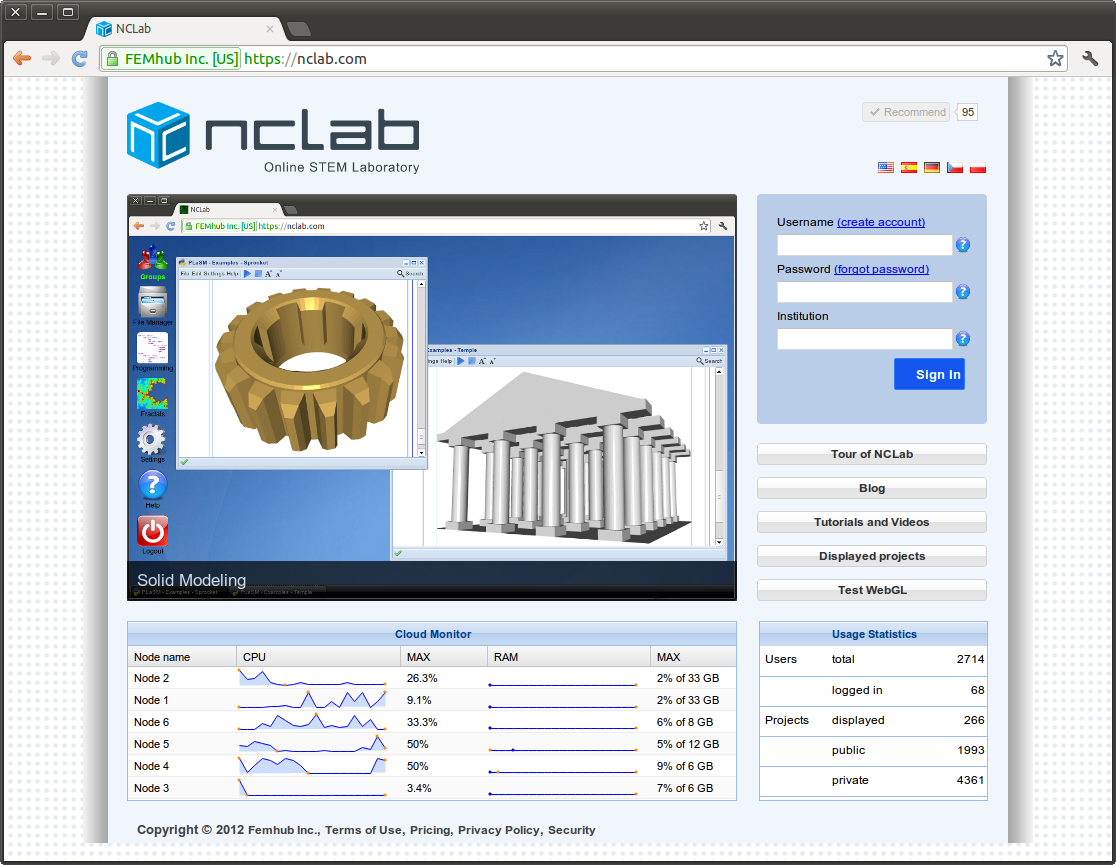
\includegraphics[width=\textwidth]{img/outside.png}
\end{center}
\vspace{-2mm}
\caption{NCLab's home page.}
\label{fig:outside}
\vspace{-0.6cm}
\end{figure}

\newpage

\subsection{Creating an Account}

In order to create a new account, click on the link "Create free account" which is next to
"Username". The following window appears:

\begin{figure}[!ht]
\begin{center}
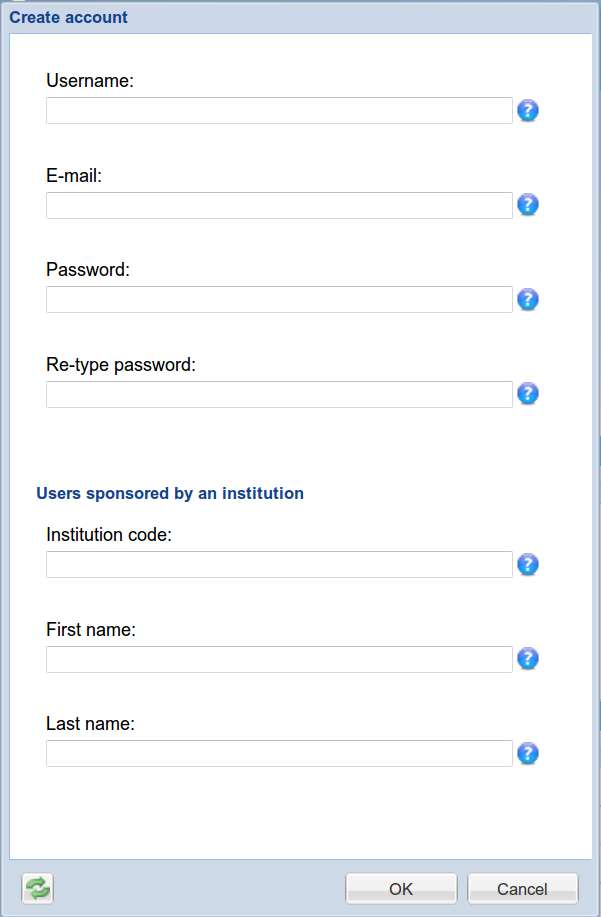
\includegraphics[width=0.45\textwidth]{img/create-account.png}
\end{center}
\vspace{-4mm}
\caption{Creating new account.}
\label{fig:creacc}
\end{figure}

\noindent
In this form, enter your preferred username, email address (to be used only if you ask
us to generate a new password for you), and password twice. Next:

\begin{itemize}
\item If you belong to an institution 
      that uses NCLab for teaching or research, you should know your institution's code. Enter it in the form, 
      along with your first and last names. Your name will be visible to an NCLab admin
      who will verify that you indeed belong to the institution.
\item If you are using NCLab for your personal hobby or self-education, for activities not 
      related to any institutional use, then leave the last three lines empty. 
\end{itemize}
After clicking OK, you are ready to login!

\subsection{After Login}

The interior of NCLab is similar to the standard computer desktop. Many users maximize 
the web browser window to make the desktop experience even more realistic.

If any member of any of your groups is in NCLab at the time you log in, the Groups icon 
will be lighted green as shown in Fig. \ref{fig:desktop}. 

\begin{figure}[!ht]
\begin{center}
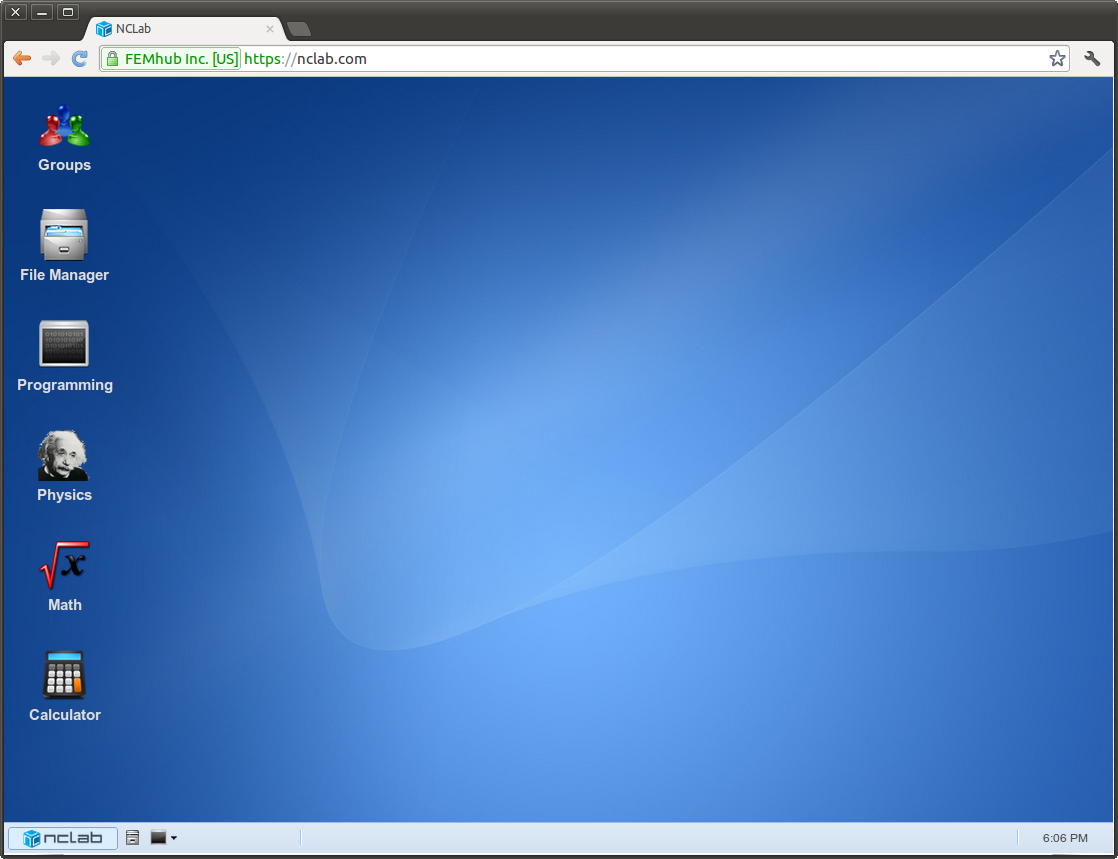
\includegraphics[width=\textwidth]{img/desktop.png}
\end{center}
%\vspace{-2mm}
\caption{NCLab desktop after login.}
\label{fig:desktop}
\end{figure}

\noindent
More about Groups and Chat will be said in a moment. First, let us briefly 
describe the other icons:

\begin{itemize}
\item File Manager is used to manage files and folders similarly to Windows Explorer. 
\item Programming Module enables programming in Karel (popular educational language for beginners),
      Python (modern programming language for advanced applications), and Javascript 
      (most popular language for web development). Additional languages are in preparation.
\item Fractal Explorer is an interactive graphical application that allows the users
      to learn about Mandelbrot and Julia fractals, and to generate beautiful fractal art.
\item Settings: Here the user can upload his/her avatar image (to be used in Groups and Chat), 
      request a new password, and adjust sound preferences.
\item Help launches a quick help about NCLab.
\item Logoff will close all applications and end the session.
\end{itemize}

\subsection{Groups and Chat}

In NCLab, users can form groups, see who is online, and chat in real time. In order to 
create a new group, click on the Groups icon. A window similar to the one shown 
in Fig. \ref{fig:groups} appears. This concrete screenshot shows four groups of the 
user "solin" -- the top one was created by Jordan, the other three by solin. The 
green light next to the last group indicates that someone in that group
is currently in NCLab. Before we go look who that is, note that you can create a
new group of your own by clicking on "New Group". In order to add people to your groups,
you need to know their usernames. The button "Who's online" allows you to see instantly 
all users in all your groups who are currently logged in. 

\begin{figure}[!ht]
\begin{center}
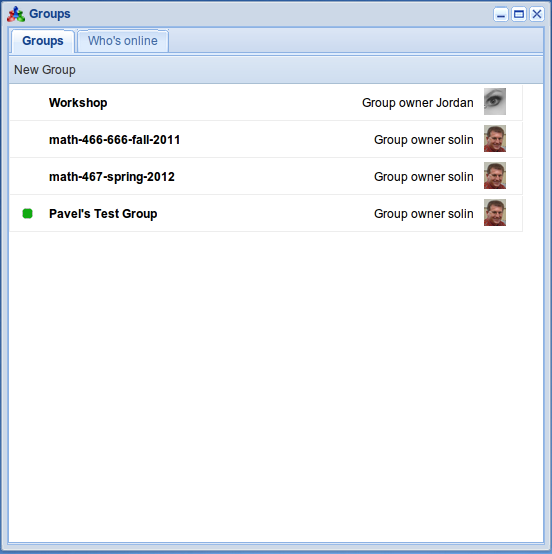
\includegraphics[width=0.5\textwidth]{img/groups.png}
\end{center}
%\vspace{-2mm}
\caption{Groups window, showing that someone in the last group is currently in NCLab.}
\label{fig:groups}
\end{figure}

\newpage
\noindent
Clicking on the last group 
reveals that the online users are Emily and Rick.
\begin{figure}[!ht]
\begin{center}
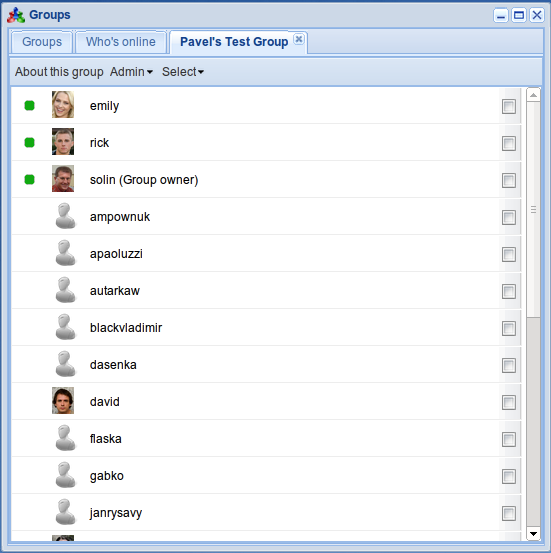
\includegraphics[width=0.5\textwidth]{img/groups-2.png}
\end{center}
%\vspace{-2mm}
\caption{Detail of the last group.}
\label{fig:groups-2}
\end{figure}

\noindent
Clicking on any user who has the green light next to him/her (except yourself),
you initiate a chat to that user. Or someone from your groups may contact you. 
The Chat window is shown in Fig. \ref{fig:chat}.

\begin{figure}[!ht]
\begin{center}
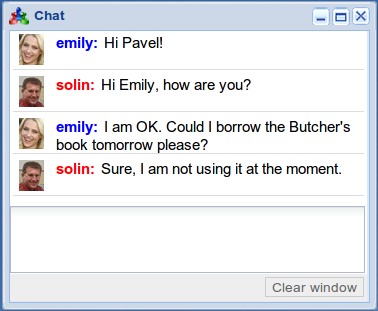
\includegraphics[width=0.4\textwidth]{img/chat.png}
\end{center}
%\vspace{-2mm}
\caption{Chat window.}
\label{fig:chat}
\end{figure}

%%%%%%%%%%%%%%%%%%%%%%%%%%%%%%%%%%%%%%%%%%%%%%%%%%%%%%%%%%%%%%%%%%%%%%%%%

\section{Using NCLab as a Calculator}

The advantage of simple calculators, such as the one shown in Fig. \ref{fig:xcalc}
is that they only have a few functions, and thus can be operated using a few buttons.

\begin{figure}[!ht]
\begin{center}
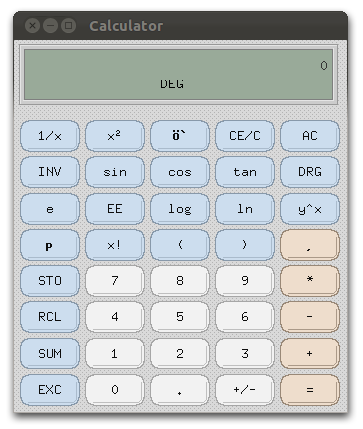
\includegraphics[width=0.4\textwidth]{img/xcalc.png}
\end{center}
%\vspace{-2mm}
\caption{Simple calculator.}
\label{fig:xcalc}
\end{figure}
\noindent
Compared to this calculator, NCLab provides an enormous functionality 
that would require thousands and thousands of buttons. So instead of buttons,
in NCLab we use simple commands to get the results we want. The language used 
to talk to NCLab is called Python. Using Python is very intuitive, 
as we shall see in a moment.

\subsection{Launching a Python Project}

Begin with clicking on the File Manager icon, which launches the File 
Manager. Next go to the menu Project in the upper-left corner. There go 
through the submenu New to Python and click. This will lanuch a new Python 
project, as illustrated in Fig. \ref{fig:python}. The same can be achieved
by clicking on the icon Programming. In the menu that appears, click on 
Python. 

\newpage

\begin{figure}[!ht]
\begin{center}
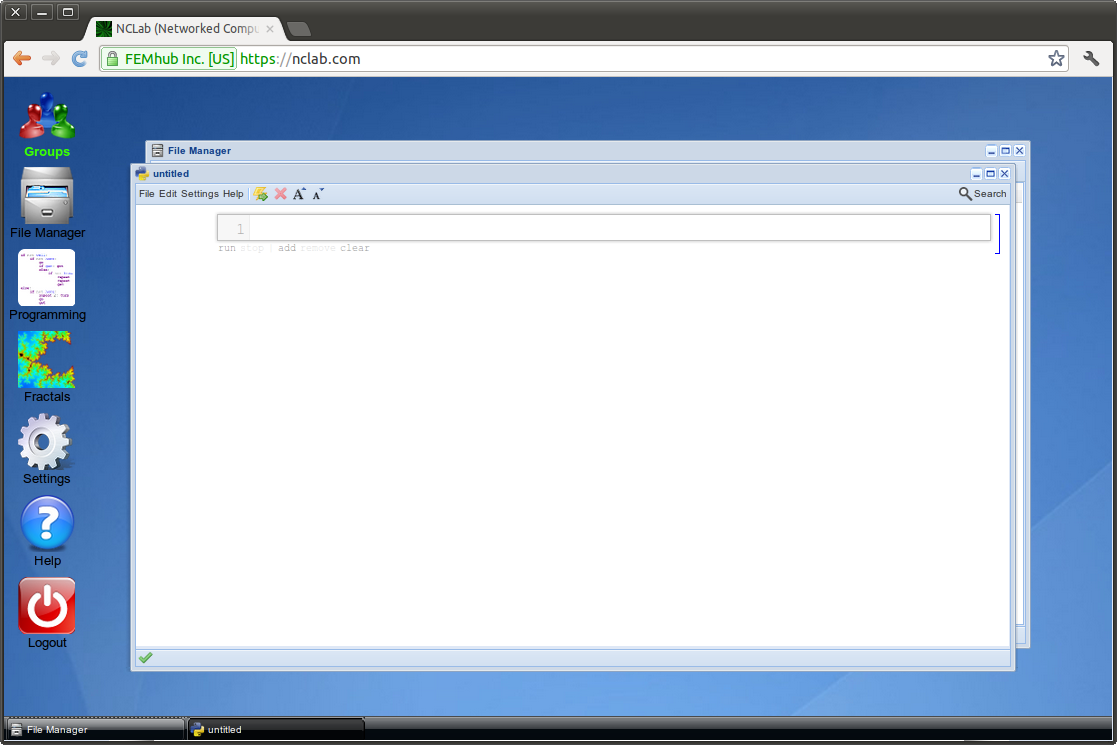
\includegraphics[width=\textwidth]{img/python.png}
\end{center}
%\vspace{-2mm}
\caption{Python project.}
\label{fig:python}
\end{figure}
\noindent
For now we will be using Python for simple math operations only,
but you could start writing an advanced Python program right 
here if you wanted. An introduction to the Python programming 
language is the subject of another NCLab tutorial.

Before we begin, it is a good idea to save your project under some 
name. This is done through the menu File and submenu Save. For 
now we can save the project in the base folder. Later you can create 
a new folder through the File Manager's menu Folder, and drag there
the project by mouse, to keep your data organized.

\subsection{Cloning Displayed Projects}

All examples that we are going to work with in the following are also available 
as Displayed Projects. This means that you can clone them by going to the
File Manager's Project menu and clicking on {\em Clone}. This will launch 
a window with many displayed projects from various areas of programming,
math and computing. Look for projects titled such as "Math - Tutorial - 1 - Simple Arithmetic",
"Math - Tutorial - 2 - Commutative, Associative and Distributive Laws", etc.
After you locate a project that you would like to clone, click on it,
and then click on the button "Clone" at the bottom of the window. This will
create exact copy of that project in your account, and you can open it 
by clicking on it in the File Manager. You can change the project in any way 
you like, the changes will not affect the original Displayed Project. 

\subsection{Simple Arithmetic (Displayed Project)}

Let's say that we have not cloned the displayed project "Math - Tutorial - 1 - Simple Arithmetic"
and instead, we prefer to start from scratch.
So your project contains a single {\em input cell}. Let's write 
something simple into it, for example "1 + 2", and click 
the link "run" right under the input cell. This sends a request to 
the cloud, it is processed there, and an answer comes back instantly. 
It is displayed in a new (yellow) {\em output cell}, as shown in 
Fig. \ref{fig:1p3}.

\begin{figure}[!ht]
\begin{center}
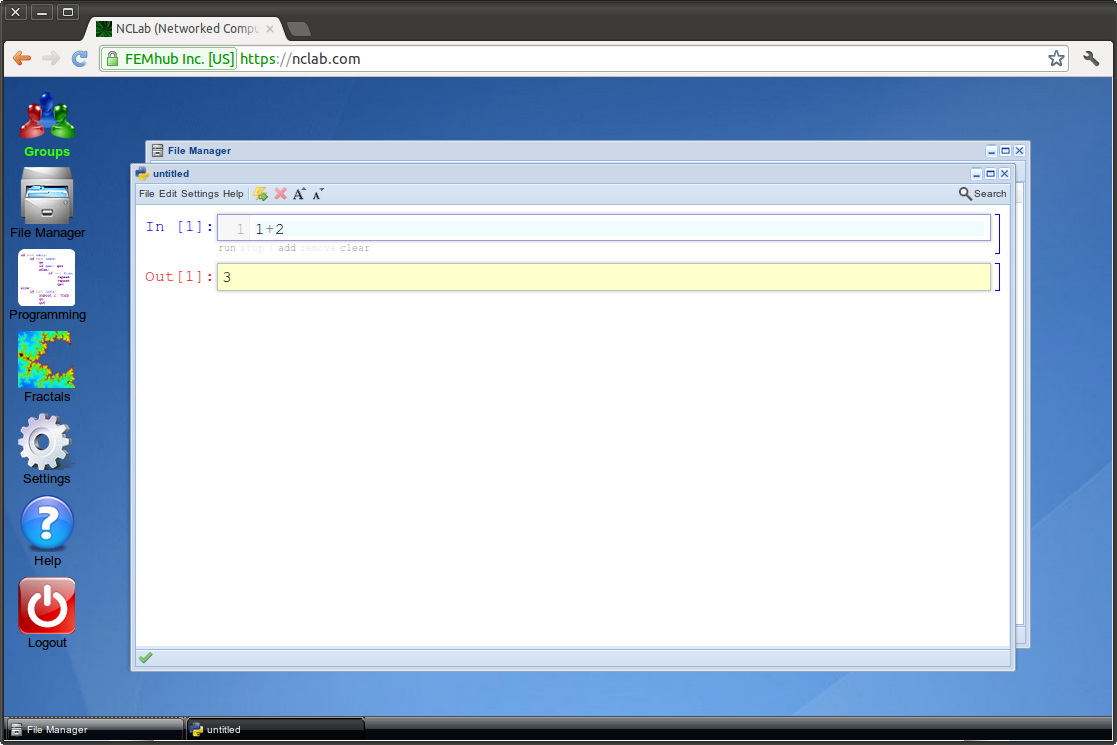
\includegraphics[width=\textwidth]{img/1p3.png}
\end{center}
%\vspace{-2mm}
\caption{Evaluating the expression "1+2".}
\label{fig:1p3}
\end{figure}
\noindent
\noindent
In addition to input and output cells, you can use {\em text cells}
to keep your project commented. This is strongly recommended. In
order to add a new text cell above the input cell, click into
the input cell, and then in menu Edit choose "New text cell above
active cell". A new text cell appears, asking you to click there to
edit its contents. Do so, and write, for example, "**Adding numbers**".
The double stars are used to make a text between them bold face. 
Then click on the link "save" right under the text cell. The result 
is shown in Fig. \ref{fig:1p3r}.

\begin{figure}[!ht]
\begin{center}
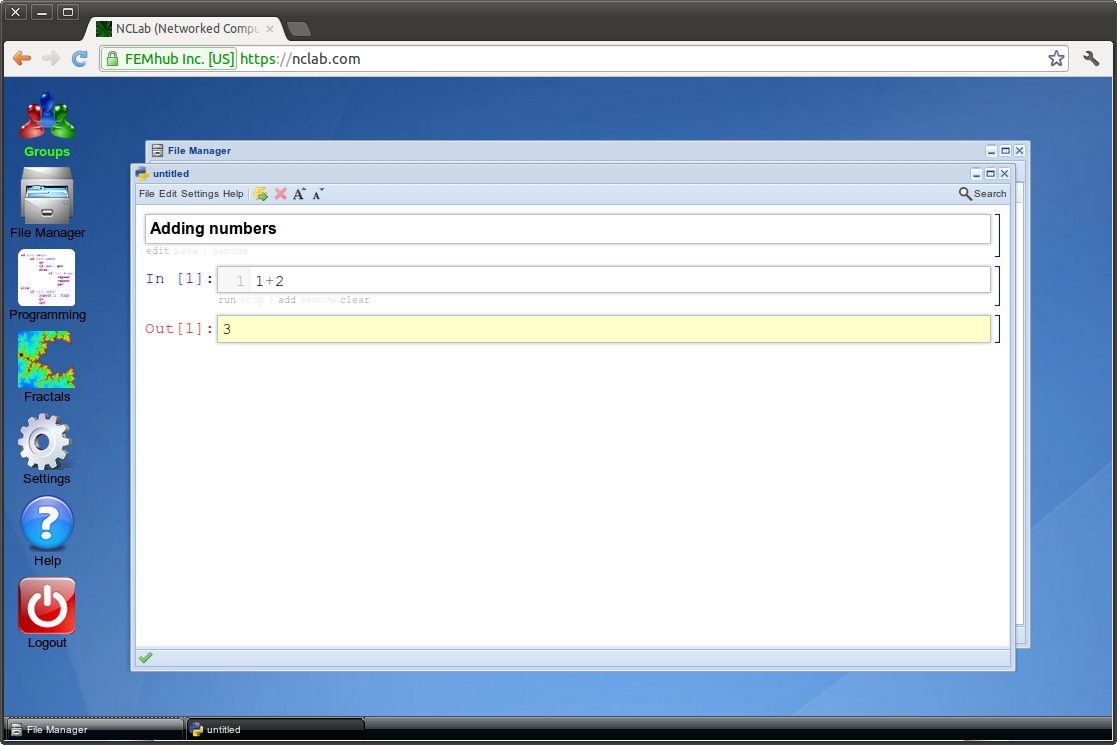
\includegraphics[width=\textwidth]{img/1p3r.png}
\end{center}
%\vspace{-2mm}
\caption{New descriptive text cell was added above the input cell.}
\label{fig:1p3r}
\end{figure}
\noindent
\noindent
If you like, you can click back into the input cell, change 
the numbers, and click the "run" link under the cell again. 
This will send a new request to the cloud and after the answer 
comes back, it is displayed in the existing output 
cell. 

Let's continue by creating a new empty input cell. To do this, click
into the previous input cell, and in menu Edit choose "New input cell 
below active cell". The new input cell will appear below the yellow 
output cell (it will never be placed between an input cell and its 
result). In there, we can experiment with other arithmetic operations 
including subtraction (try for example "5 - 3"), multiplication 
(try for example "3.21 * 7.45"). The results are shown in Fig. \ref{fig:1p3r2}.

\begin{figure}[!ht]
\begin{center}
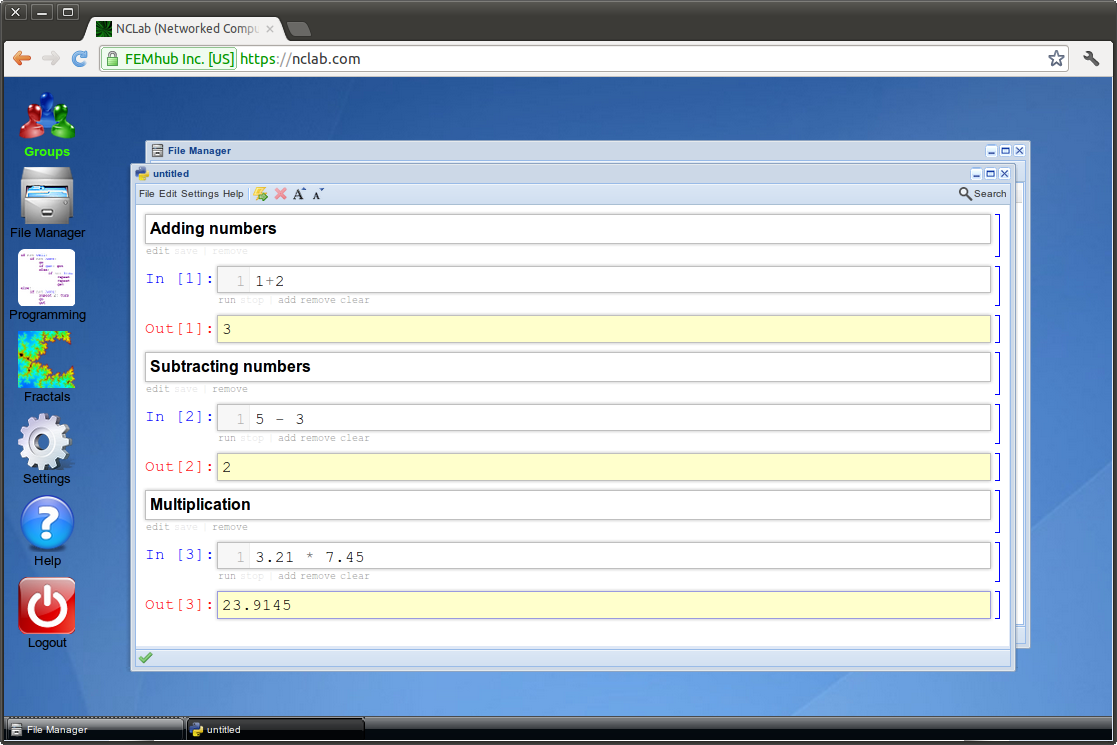
\includegraphics[width=\textwidth]{img/1p3r2.png}
\end{center}
%\vspace{-2mm}
\caption{Subtraction and multiplication.}
\label{fig:1p3r2}
\end{figure}
\noindent
At this point we may go to menu Edit and click on 
"Remove all output" -- this will free up some space.\\

\noindent
{\em BEWARE - Division of Two integers Always is an Integer}\\

Numbers such as "12" or "5" are integers. In Python, as well as 
in other major programming languages, the {\bf result of division of 
two integers always is an integer}. This means that anything beyond 
the decimal point in the result is erased! Let us see this in reality:

\newpage
\begin{figure}[!ht]
\begin{center}
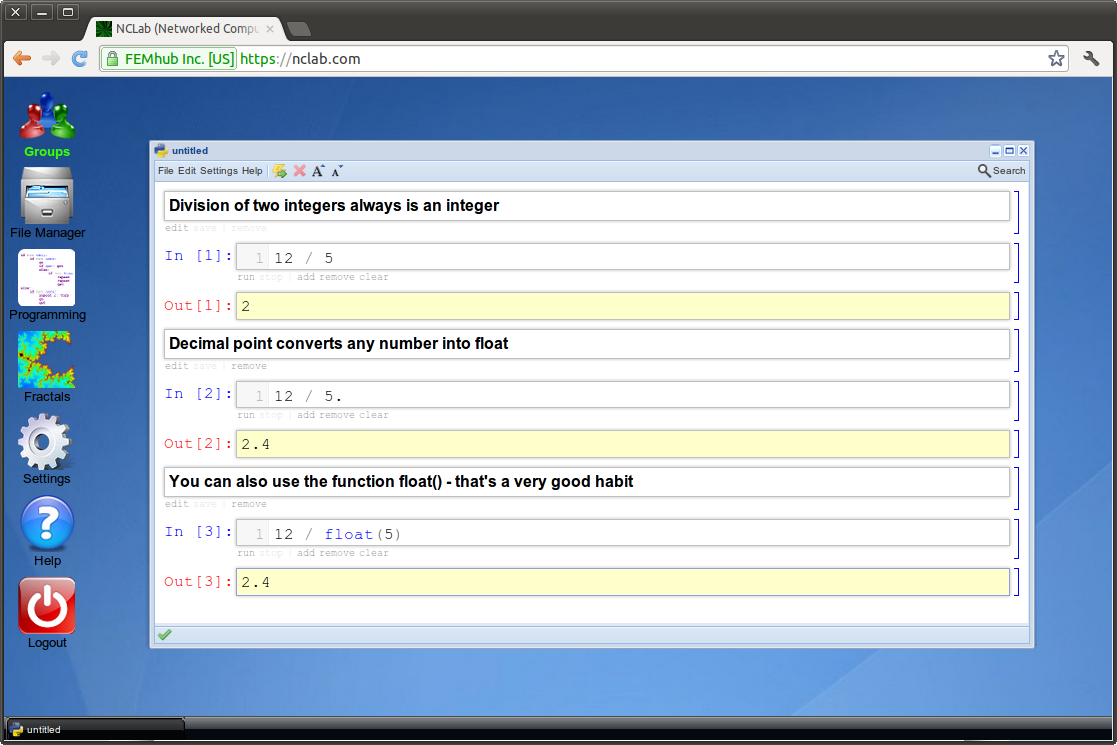
\includegraphics[width=\textwidth]{img/div1.png}
\end{center}
%\vspace{-2mm}
\caption{Division of two integers always is an integer \& two ways to make division safe.}
\label{fig:div1}
\end{figure}
\noindent
Fig. \ref{fig:div1} shows that evaluating simply 12/5 leads to a wrong result. An easy fix is 
to convert one of the numbers into a float by appending a decimal point to it. Still
another way, also shown in  Fig. \ref{fig:div1}, is to convert one of the numbers into a float 
via the function {\tt float()}. The latter approach works even for the division of variables "a/b"
where one may not know exactly whether they are integers or floats. Whenever at least 
one of the numbers if float, the result is a float. \\

\noindent
If you are a mathematician -- yes, you are right. we forgot to discuss division by zero. 
It is useful to see how NCLab reports errors, so let's do it!

\newpage
\begin{figure}[!ht]
\begin{center}
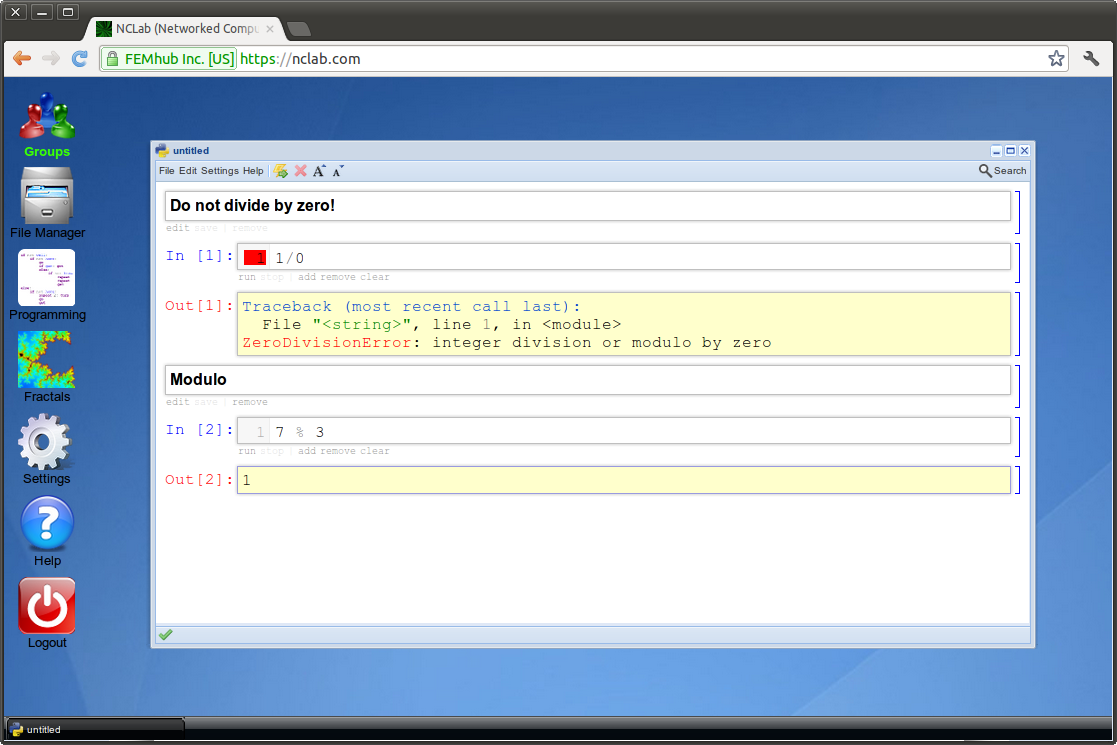
\includegraphics[width=\textwidth]{img/divzero.png}
\end{center}
%\vspace{-2mm}
\caption{Error is reported when dividing by zero.}
\label{fig:divzero}
\end{figure}
\noindent
Since the error message in Fig. \ref{fig:divzero} mentioned modulo, we added there one more 
input cell demonstrating how modulo is done -- using the \% symbol.

\subsection{Commutative, Associative and Distributive Laws (Displayed Project)}

The validity of these laws can be verified easily on examples. One just enters
a code similar to 

\begin{verbatim}
a = 2
b = 3
print "a + b =", a + b
print "b + a =", b + a
\end{verbatim}
and clicks on the link "run" under the input cell. The output 
is shown in Fig. \ref{fig:commut}. 

\begin{figure}[!ht]
\begin{center}
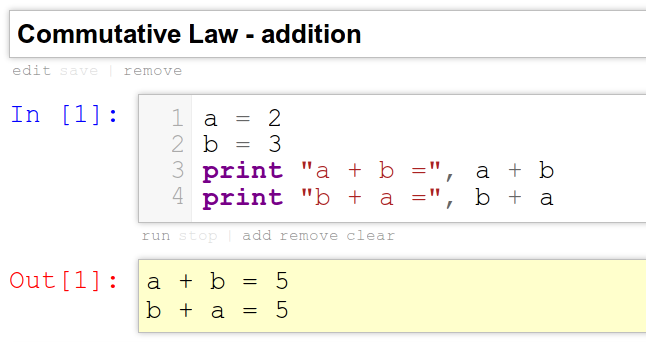
\includegraphics[width=0.6\textwidth]{img/commut.png}
\end{center}
\vspace{-4mm}
\caption{Commutative Law holds!}
\label{fig:commut}
%\vspace{-6mm}
\end{figure}




\subsection{List of Elementary Functions  (Displayed Project)}

In order to calculate square roots, exponentials, sins, cosins, tangents, and all other 
simple functions, the best way is to import Numpy as shown in Fig. \ref{fig:fns}. Numpy 
is a standard Python library for numerical computations.

\begin{figure}[!ht]
\begin{center}
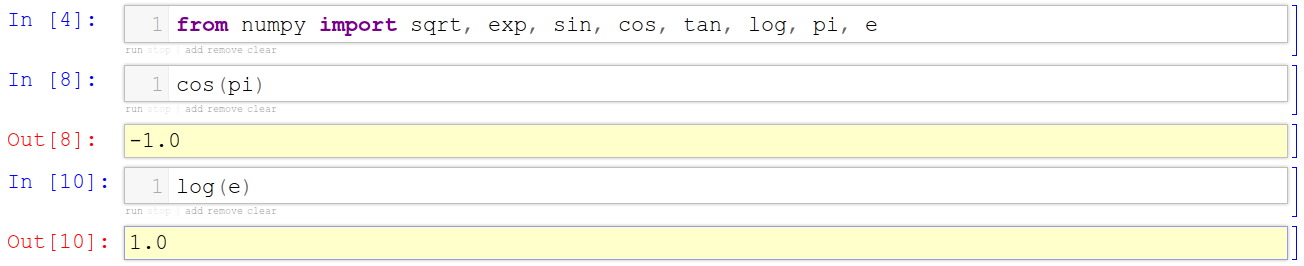
\includegraphics[width=\textwidth]{img/fns.png}
\end{center}
\vspace{-4mm}
\caption{Importing Numpy and using elementary functions.}
\label{fig:fns}
%\vspace{-6mm}
\end{figure}

\newpage
\noindent
Elementary functions that one can import from Numpy include:\\

%{\small
\begin{center}
\begin{tabular}{|l|l|}
\hline
abs($x$) &  absolute value of $x$\\
arccos($x$) &  inverse cosine of $x$ \\
arccosh($x$) &  inverse hyperbolic cosine of $x$ \\
arcsin($x$) & inverse sine of $x$ \\
arcsinh($x$) & inverse hyperbolic sine of $x$ \\
arctan($x$) & inverse tangent of $x$ \\
arctanh($x$) & inverse hyperbolic tangent of $x$ \\
arctan2($x_1$, $x_2$) & arc tangent of $x_1/x_2$ choosing the quadrant correctly \\
cos($x$) & cosine of $x$ \\
cosh($x$) & hyperbolic tangent of $x$ \\
exp($x$) & $e^x$ \\
log($x$) & natural logarithm of $x$ \\
pow($a$, $b$) & $a^b$ (same as "a**b")\\
sin($x$) & sine of $x$ \\
sinh($x$) & hyperbolic sine of $x$ \\
sqrt($x$) & square root of $x$ \\
tan($x$) & tangent of $x$\\
tanh($x$) & hyperbolic tangent of $x$ \\
\hline
\end{tabular}
\end{center}
%}
\vspace{4mm}
\noindent
For a complete overview of functions provided by Numpy we recommend the 
web page \\ {\tt http://www.scipy.org/Numpy\_Functions\_by\_Category}.


\subsection{Using Built-In Help}

Whenever you are unsure about a command, you can enter the 
command followed by a questionmark, and click on "run". This will 
display help that is available for that command, and in many cases also
examples of its correct use. This is illustrated for the command 
"arctan2" in Fig. \ref{fig:help}.

\newpage

\begin{figure}[!ht]
\begin{center}
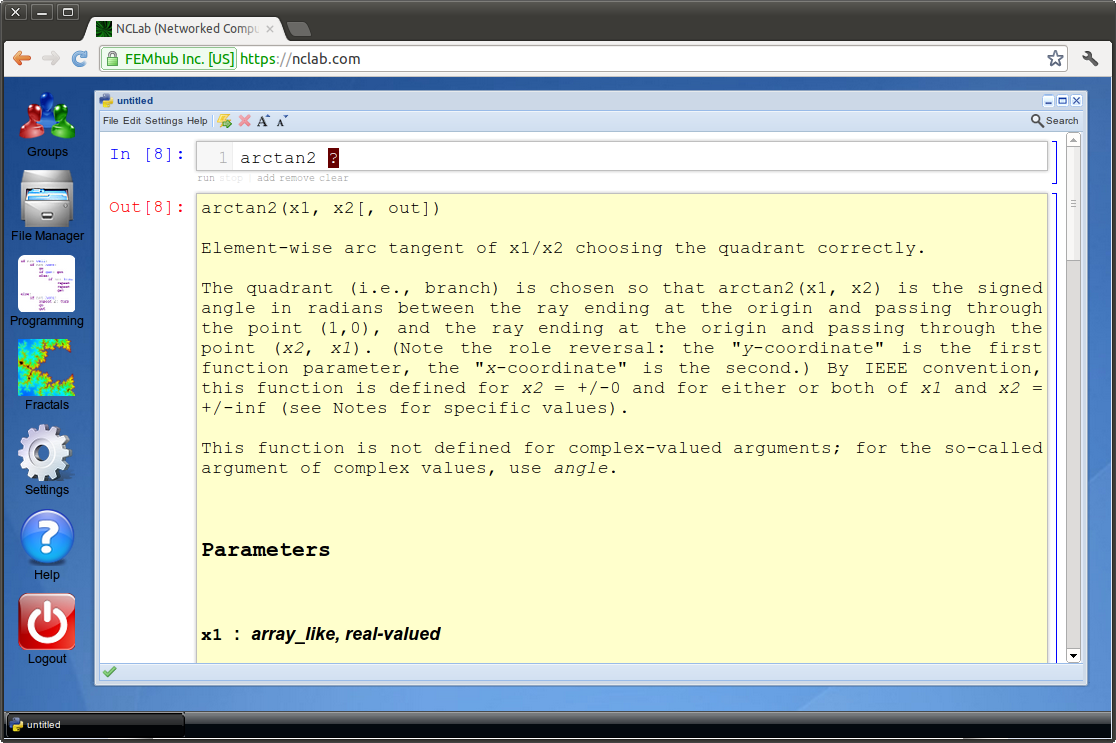
\includegraphics[width=\textwidth]{img/help.png}
\end{center}
\vspace{-2mm}
\caption{Typing a keyword followed by '?' and clicking on "run" invokes built-in help.}
\label{fig:help}
%\vspace{-1cm}
\end{figure}

\subsection{Plotting Functions of One Variable (Displayed Project)}\label{plotting}

Plotting can be done via the Pylab library. Pylab is a standard Python library that is 
superior in almost every way to MATLAB (expensive commercial product whose usage is 
quite similar to what we are doing here). The Pylab {\tt plot} command takes two
lists: $x$-coordinates and $y$-coordinates of points on a curve. Between the 
points, the curve is interpolated linearly. Let us illustrate this on a simple 
example with just five points [0, 0], [1, 2], [2, 0.5], [3, 2.5] and [4, 0]:

\begin{verbatim}
from pylab import *
x = [0,0, 1.0, 2.0, 3.0, 4.0]
y = [0.0, 2.0, 0.5, 2.5, 0]
clf()
plot(x, y)
lab.show()
\end{verbatim}
\newpage
\noindent
The commands {\tt clf()}, {\tt plot()} and {\tt lab.show()} do clear the canvas, 
plot the graph, and show the graph, respectively.
The output is shown in Fig. \ref{fig:plot}.


\begin{figure}[!ht]
\begin{center}
\hbox{}
\hspace{-6mm}
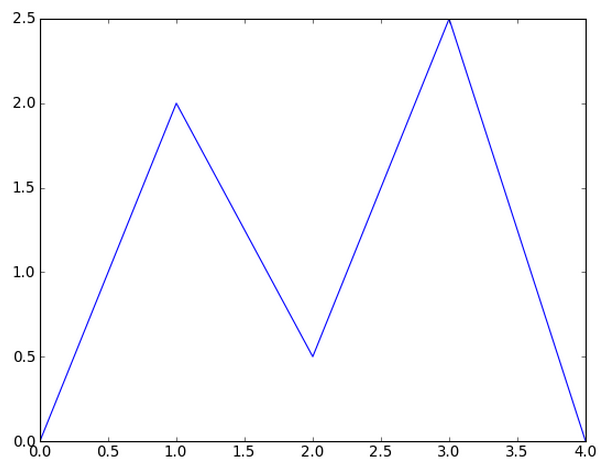
\includegraphics[width=0.56\textwidth]{img/plot.png}
\end{center}
\vspace{-2mm}
\caption{Piecewise-linear curve with five points.}
\label{fig:plot}
%\vspace{-1cm}
\end{figure}
\noindent
In the following we will discuss more options and show some useful techniques.
Let's say, for example, that we want to plot the function $f(x) = \sin(x)$
in the interval $(0, 2\pi)$. The array of $x$-coordinates of equidistant points 
between 0 and $\pi$ with step 0.05 can be created easily using the command {\tt arange}:

\begin{verbatim}
from numpy import *
x = arange(0, 2*pi, 0.05)
\end{verbatim}
Changing the step size will change the resolution - with a smaller step the resolution will 
be finer and vice-versa. Next, the array of $y$-coordinates of the points is obtained via

\begin{verbatim}
y = sin(x)
\end{verbatim}
The last part we already know:

\begin{verbatim}
clf()
plot(x, y)
lab.show()
\end{verbatim}
\noindent
The output is shown in Fig. \ref{fig:plot1}.

\newpage

\begin{figure}[!ht]
\begin{center}
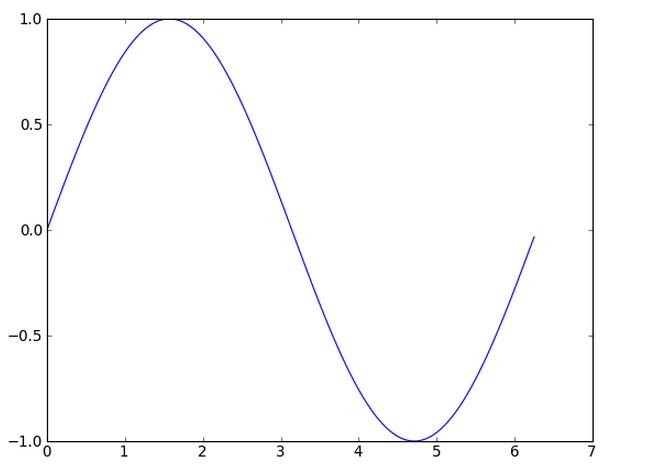
\includegraphics[width=0.6\textwidth]{img/plot1.png}
\end{center}
\vspace{-6mm}
\caption{Plotting $\sin(x)$ in interval $(0, 2\pi)$ with subdivision step 0.05.}
\label{fig:plot1}
\vspace{-2mm}
\end{figure}
\noindent
The plot can be made nicer by adding a label, and also the color 
and the line style can be changed. Let us start with adding a label:

\begin{verbatim}
lb = "Solid blue line"
plot(x, y, 'b-', label = lb)
legend()
lab.show()
\end{verbatim}
The output is shown in Fig. \ref{fig:plot2}.

\begin{figure}[!ht]
\begin{center}
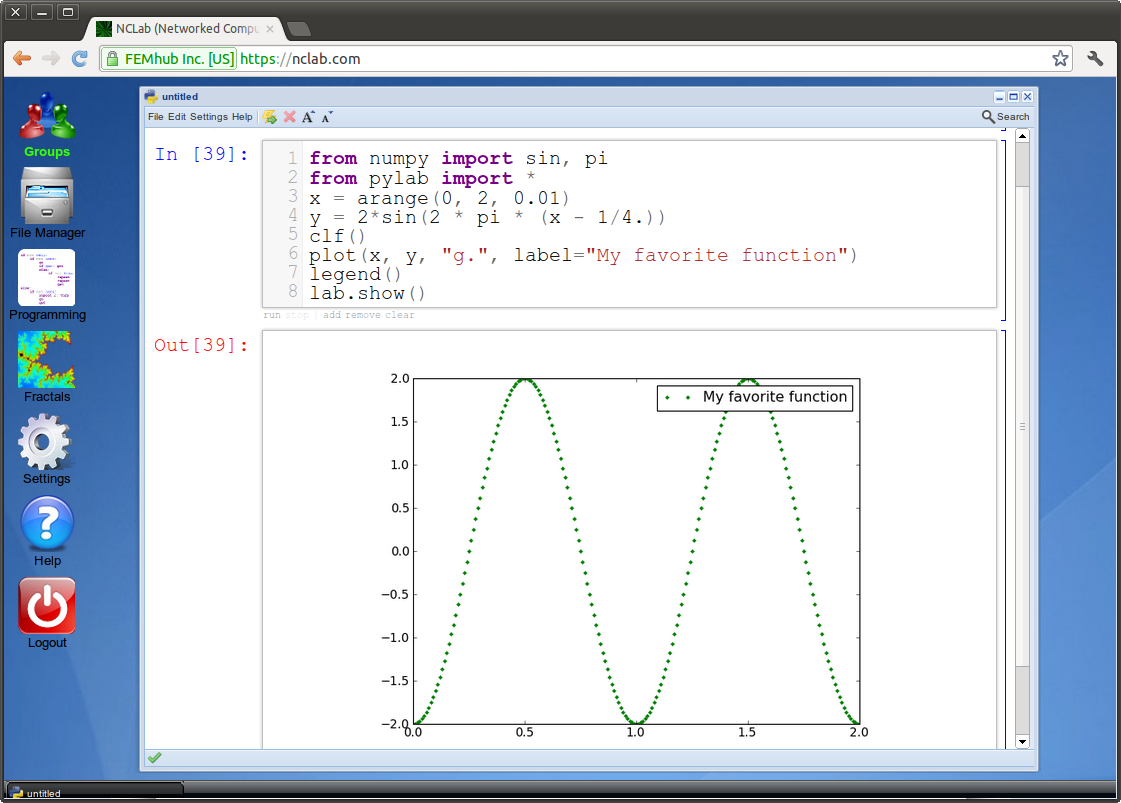
\includegraphics[width=0.6\textwidth]{img/plot2.png}
\end{center}
\vspace{-6mm}
\caption{Adding a label.}
\label{fig:plot2}
\vspace{-1cm}
\end{figure}
\newpage

\noindent
Next let us change the color to red and line style to dashed: 

\begin{verbatim}
lb = "Dashed red line"
clf()
plot(x, y, 'r--', label = lb)
legend()
lab.show()
\end{verbatim}
The output is shown in Fig. \ref{fig:plot3}.



\begin{figure}[!ht]
\begin{center}
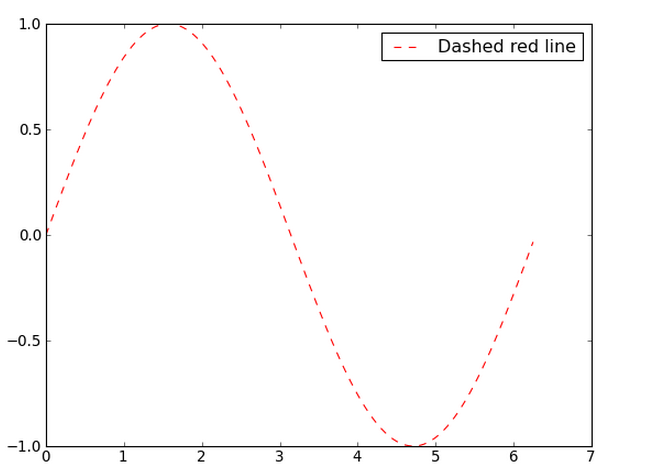
\includegraphics[width=0.6\textwidth]{img/plot3.png}
\end{center}
\vspace{-2mm}
\caption{Same graph using dashed red line.}
\label{fig:plot3}
\end{figure}
\noindent
The graph can be plotted using green color and small dots rather than 
a solid or dashed line:

\begin{verbatim}
lb = "Dashed red line"
clf()
plot(x, y, 'g.', label = lb)
legend()
lab.show()
\end{verbatim}
The output is shown in Fig. \ref{fig:plot4}.

\newpage

\begin{figure}[!ht]
\begin{center}
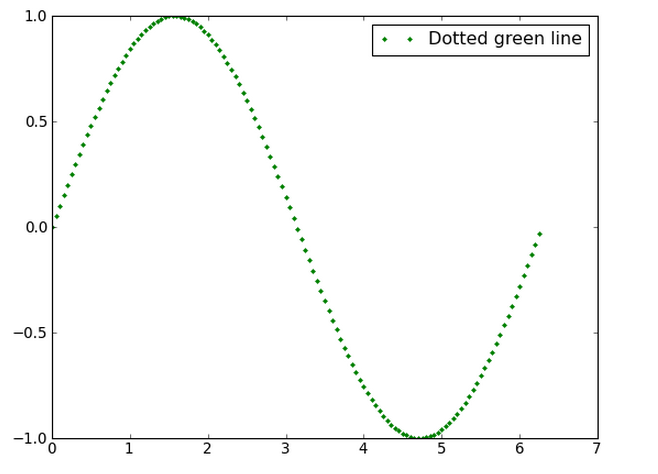
\includegraphics[width=0.6\textwidth]{img/plot4.png}
\end{center}
\vspace{-6mm}
\caption{Same graph using dotted green line.}
\label{fig:plot4}
\vspace{-5mm}
\end{figure}
\noindent
Last let us stay with green color but make the dots larger:

\begin{verbatim}
lb = "Dashed red line"
clf()
plot(x, y, 'go', label = lb)
legend()
lab.show()
\end{verbatim}
The output is shown in Fig. \ref{fig:plot5}.

\begin{figure}[!ht]
\begin{center}
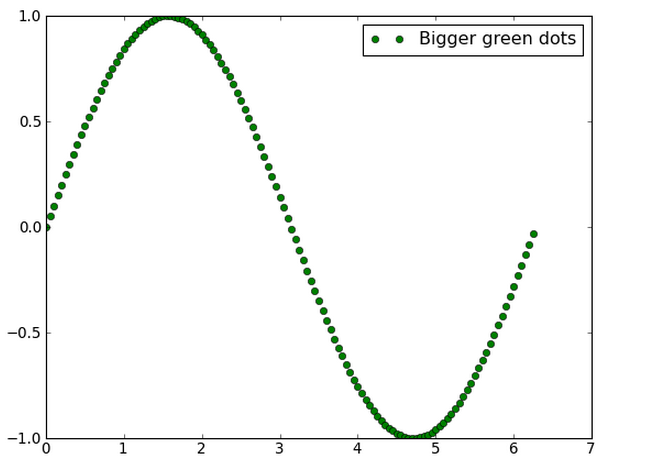
\includegraphics[width=0.6\textwidth]{img/plot5.png}
\end{center}
\vspace{-6mm}
\caption{Same graph using large green dots.}
\label{fig:plot5}
\vspace{-4mm}
\end{figure}
\noindent
For a complete list of options available for the {\tt plot} command, 
visit the Pylab page {\tt http:// www.scipy.org/PyLab}.

\subsection{Plotting General Planar Curves (Displayed Project)}

The concept of plotting based on two arrays of $x$ and $y$ coordinates
allows us to do much more than only plot graphs of functions of one variable.
We can easily plot more general curves such as circles, spirals and others.
Let us illustrate this on a spiral that this parameterized 
by 
$$
x(t) = t \cos(t), \ \ \ \ 
y(t) = t \sin(t)
$$ 
in the interval $(0, 10)$ for $t$. The complete code is

\begin{verbatim}
from pylab import *
from numpy import *
t = arange(0, 10, 0.05)
x = t*cos(t)
y = t*sin(t)
clf()
plot(x, y)
lab.show()
\end{verbatim}
The output is shown in Fig. \ref{fig:plot6}.

\begin{figure}[!ht]
\begin{center}
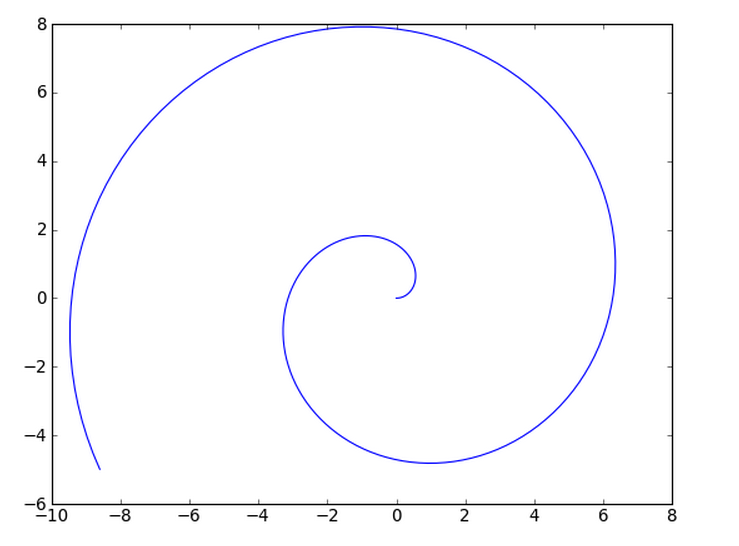
\includegraphics[width=0.6\textwidth]{img/plot6.png}
\end{center}
\vspace{-6mm}
\caption{.}
\label{fig:plot6}
\vspace{-4mm}
\end{figure}
\noindent


\subsection{Plotting Functions of Two Variables (Displayed Project)}

For this functionality, your browser has to support WebGL (most of modern browsers do, 
with the exception of Internet Explorer). NCLab offer the following simple way to plot 
functions of two variables:

{\small
\begin{verbatim}
from numpy import sin, sqrt, arctan

# Define intervals on the x and y axes.
x0 = 0.0
x1 = 10.0
y0 = 0.0
y1 = 10.0

# Define the corresponding divisions.
nx = 100
ny = 100

# Render the surface using WebGL.
lab.surface((x0, x1, nx), (y0, y1, ny), lambda x, y: sin(sqrt(x**2 + y**2)))
\end{verbatim}
}

\begin{figure}[!ht]
\begin{center}
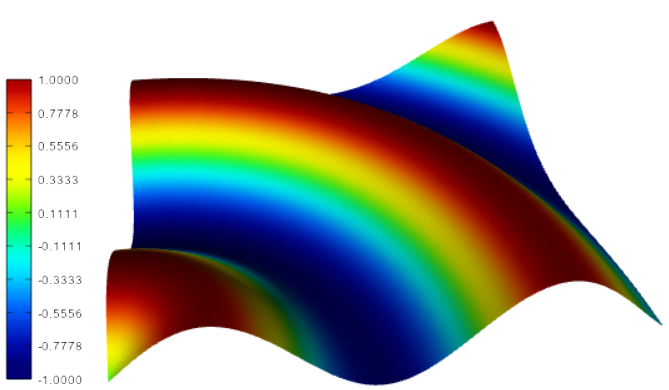
\includegraphics[width=0.8\textwidth]{img/webgl.png}
\end{center}
\vspace{-2mm}
\caption{Plotting functions of two variable.}
\label{fig:webgl}
%\vspace{-1cm}
\end{figure}

%%%%%%%%%%%%%%%%%%%%%%%%%%%%%%%%%%%%%%%%%%%%%%%%%%%%%%%%%%%%%%%%%%%%%%%%%

\section{High School Algebra (Displayed Project)}\label{algebra}

In the following we will be working with functions, polynomials, fractions, and such.
Here are a few useful tricks.

\subsection{Entering an expression}
Algebraic expressions are represented using text strings that resemble 
computer code (well, they {\em are} computer code). For example, the expression 
$$
  (x + y)^2 (x + 1)
$$ 
needs to be entered as
\begin{verbatim}
(x + y)**2 * (x + 1)
\end{verbatim}
Longer expressions, when entered as one piece, may not be all that well readable. For example,
$$
\frac{(x + y)^2 (x + 1) + \frac{(x-5)(x-3)}{(x-4)^2} + (x + y)(x - 2)(x + y)^3}{(x-1)(x+2))}
$$ 
would be entered as 
\begin{verbatim}
((x + y)**2 * (x + 1) + (x - 5)*(x - 3)/(x - 4)**2 
+ (x + y)*(x - 2)*(x + y)**3)/((x - 1)*(x + 2))
\end{verbatim}
The same can be written more elegantly using simpler expressions:
\begin{verbatim}
A = (x + y)**2 * (x + 1)
B = (x - 5)*(x - 3)/(x - 4)**2
C = (x + y)*(x - 2)*(x + y)**3
D = (x - 1)*(x + 2)
(A + B + C)/D
\end{verbatim}

\subsection{Pretty printing}
An expression can be printed in a prettier way using the command {\tt pprint} (stands for {\em pretty print}):
\begin{verbatim}
pprint( (x+y)**2 * (x + 1) )
\end{verbatim}
Result:
\begin{verbatim}
       2
(x + y)  * (1 + x)
\end{verbatim}
Another example would be
\begin{verbatim}
pprint((x**2 + y**2 + z**2)/(x*y*z))
\end{verbatim}
Result:
\begin{verbatim}
 2   2   2
x + y + z
----------
  x*y*z   
\end{verbatim}
All examples in this section are available in the displayed project 
"Math - Tutorial - 07 - High School Algebra". You can clone the project into 
your user account via the menu Project $\rightarrow$ Clone in the File 
Manager, and experiment with the examples on your own.

For algebra, calculus, differential equations and related symbolic calculations 
we import the Sympy library:

\begin{verbatim}
from sympy import *
\end{verbatim}
At the beginning, we need to declare the names of symbolic variables (to distinguish 
them from constants). For example, if we know that we are going to work with functions 
of $x$, $y$ and/or $z$, we may declare these symbols at once:
\begin{verbatim}
x, y, z = symbols("xyz")
\end{verbatim}
With this, we are ready to go!

\subsection{Expanding expressions}

To expand an expression, we use the command {\tt expand}:
\begin{verbatim}
A = expand( (x+y)**2 * (x+1) )
pprint(A)
\end{verbatim}
Result:
\begin{verbatim}
         2    2      2        2    3
2*x*y + x  + y  + x*y  + 2*y*x  + x 
\end{verbatim}

\subsection{Simplifying expressions}

In order to simplify an expression, we use the command {\tt simplify}:
\begin{verbatim}
simplify( 1/x + (x*sin(x) - 1)/x )
\end{verbatim}
Result:
\begin{verbatim}
sin(x)
\end{verbatim}
Another example:
\begin{verbatim}
A = simplify( 1/x + 1/y + 1/z )
pprint(A)
\end{verbatim}
Result:
\begin{verbatim}
x*y + x*z + y*z
---------------
     x*y*z     
\end{verbatim}

\subsection{Factoring polynomials}

This is done using the command {\tt factor}:
\begin{verbatim}
factor(x**4 - 3*x**2 + 1)
\end{verbatim}
Result:
\begin{verbatim}
(1 + x - x**2)*(1 - x - x**2)
\end{verbatim}
In order to get a more thorough factorization, one can do:
\begin{verbatim}
factor(x**4 - 3*x**2 + 1, modulus=5)
\end{verbatim}
Result:
\begin{verbatim}
(2 + x)**2*(2 - x)**2
\end{verbatim}


\subsection{Calculating roots of polynomials}

The command {\tt roots} can be used to calculate all roots of a polynomial:
\begin{verbatim}
roots(-15 - 13*x + 3*x**2 + x**3, x)
\end{verbatim}
Result:
\begin{verbatim}
{-5: 1, -1: 1, 3: 1}
\end{verbatim}
It also works in the complex case:
\begin{verbatim}
roots(x**2 + 1, x)
\end{verbatim}
Result:
\begin{verbatim}
{-I: 1, I: 1}
\end{verbatim}


\subsection{Solving linear equations and systems}

In order to solve an equation or a system of equations, we use the command {\tt solve}.
For example, in order to solve the equation 
$$
3x - 4 - 2 = 0,
$$
we type:
\begin{verbatim}
solve(3*x - 4 - 2, [x])
\end{verbatim}
Result:
\begin{verbatim}
[2]
\end{verbatim}
\noindent
Here is an example for a system of two equations:
\begin{verbatim}
solve([x + 5*y - 2, -3*x + 6*y - 15], [x, y])
\end{verbatim}
Result:
\begin{verbatim}
{x: -3, y: 1}
\end{verbatim}
And one more example for a system of three equations:
\begin{verbatim}
solve([x + 5*y - z - 2, -3*x + 6*y + z - 15, x + y + z], [x, y, z])
\end{verbatim}
Result:
\begin{verbatim}
{x: -3, y: 1}{x: -40/17, y: 19/17, z: 21/17}
\end{verbatim}
\noindent

\subsection{Solving polynomial equations}

Nonlinear equations can be solved using the same command {\tt solve}.
For example, in order to solve the equation 
$$
3x^3 - 4 = 2,
$$
we type:
\begin{verbatim}
A = solve([3*x**3 - 4 - 2], [x])
pprint(A)
\end{verbatim}
Result:
\begin{verbatim}
              3 ___   ___   3 ___         3 ___   ___   3 ___   
  3 ___     I*\/ 2 *\/ 3    \/ 2        I*\/ 2 *\/ 3    \/ 2    
[(\/ 2 ,), (------------- - -----,), (- ------------- - -----,)]
                  2           2               2           2     
\end{verbatim}

\subsection{Solving transcendental equations}

For example, let us solve the equation
$$
e^x + 1 = 0.
$$
This is done as follows:
\begin{verbatim}
solve(exp(x) + 1, x)
\end{verbatim}
Result:
\begin{verbatim}
[pi*I]
\end{verbatim}

%%%%%%%%%%%%%%%%%%%%%%%%%%%%%%%%%%%%%%%%%%%%%%%%%%%%%%%%%%%%%%%%%%%%%%%%%

\section{Calculus (Displayed Project)}

All examples in this section are available in the displayed project 
"Math - Tutorial - 08 - Calculus". You can clone the project into 
your user account via the menu Project $\rightarrow$ Clone in the File 
Manager, and experiment with the examples on your own.

Let us remind the reader that for symbolic calculations we need to 
import Sympy, and declare symbolic variables:
\begin{verbatim}
from sympy import *
x, y, z  = symbols("xyz")
\end{verbatim}

\subsection{Calculating limits}

\noindent
For example, let us show how to calculate the limit
$$
\lim_{x \rightarrow 0} \frac{\sin(x) - x}{x^3}.
$$
This is done using the command {\tt limit}:
\begin{verbatim}
limit((sin(x) - x)/x**3, x, 0)
\end{verbatim}
Result:
\begin{verbatim}
-1/6
\end{verbatim}
We can also calculate limits as $x \rightarrow \infty$. Infinity is represented 
in Sympy as {\tt oo}:
\begin{verbatim}
limit((x + sin(1/x))/(1 + x^2), x, oo)
\end{verbatim}
Result:
\begin{verbatim}
0
\end{verbatim}

\subsection{Calculating derivatives from definition}

One can use the {\tt limit} command to calculate derivatives:
\begin{verbatim}
limit((tan(x+y)-tan(x))/y, y, 0)
\end{verbatim}
Result:
\begin{verbatim}
1 + tan(x)**2
\end{verbatim}

\subsection{Differentiation}

Taking derivatives is very simple using the command {\tt diff}. For example:
\begin{verbatim}
diff(sin(x), x)
\end{verbatim}
Result:
\begin{verbatim}
cos(x)
\end{verbatim}
Another example:
\begin{verbatim}
result = diff(log(x) / x**2, x)
pprint(result)
\end{verbatim}
Result:
\begin{verbatim}
  2*log(x)   1 
- -------- + --
      3       3
     x       x 
\end{verbatim}

\subsection{Higher derivatives}

Taking higher derivatives is also simple:
\begin{verbatim}
diff(sin(2*x), x, 2)
\end{verbatim}
Result:
\begin{verbatim}
-4*sin(2*x)
\end{verbatim}

\subsection{Finding local extrems of functions}

We have shown in Paragraph \ref{plotting} how to plot a function of one variable. 
Of course, one can differentiate the function and plot it. Let's say, for example, that 
we want to plot the derivative of the function $f(x) = 2\sin(2\pi(x - 1/4))$
in the interval $(0, 2)$. This is done as follows:
\begin{verbatim}
from numpy import sin, pi
from pylab import *
x = arange(0, 2, 0.01)
y = diff(2*sin(2 * pi * (x - 1/4.)), x)
clf()
plot(x, y)
lab.show()
\end{verbatim}
Analogously, we can differentiate the function twice and look for inflection points:
\begin{verbatim}
from numpy import sin, pi
from pylab import *
x = arange(0, 2, 0.01)
y = diff(2*sin(2 * pi * (x - 1/4.)), x, 2)
clf()
plot(x, y)
lab.show()
\end{verbatim}
Indeed it is possible to calculate the extrema using the function {\tt solve}
as we have shown in Section \ref{algebra}.

\subsection{Taylor series expansion}

For this we use the {\tt series} command:
\begin{verbatim}
A = 1/cos(x)
result = A.series(x, 0, 7)
pprint(result)
\end{verbatim}
Result:
\begin{verbatim}
     2      4       6          
    x    5*x    61*x           
1 + -- + ---- + ----- + O(x**7)
    2     24     720           
\end{verbatim}

\subsection{Integration}

For example, let us calculate 
$$
\int \frac{1}{\sqrt{1 + 2x^2}}\, \mbox{d} x.
$$
This is done as follows:
\begin{verbatim}
result = integrate(1/sqrt(1 + 2*x**2), x)
pprint(result)
\end{verbatim}
Result:
\begin{verbatim}
  ___      /    ___\
\/ 2 *asinh\x*\/ 2 /
--------------------
         2      
\end{verbatim}

\subsection{Computing definite integrals}

For example, let us calculate
$$
\int_0^{\infty} e^{-x}\, \mbox{d} x.
$$
This is done as follows:
\begin{verbatim}
integrate(exp(-x), (x, 0, oo))
\end{verbatim}
Result:
\begin{verbatim}
pi**(1/2)
\end{verbatim}
Another example:
\begin{verbatim}
integrate(cos(x), (x, -pi/2, pi/2))
\end{verbatim}
Result:
\begin{verbatim}
2
\end{verbatim}

\subsection{Computing improper integrals}

For example, let us calculate
$$
\int_{-\infty}^{\infty} e^{-x^2}\, \mbox{d} x.
$$
This is done as follows:
\begin{verbatim}
integrate(exp(-x**2), (x, -oo, oo))
\end{verbatim}
Result:
\begin{verbatim}
pi**(1/2)
\end{verbatim}

%%%%%%%%%%%%%%%%%%%%%%%%%%%%%%%%%%%%%%%%%%%%%%%%%%%%%%%%%%%%%%%%%%%%%%%%%

\section{Matrix Algebra (Displayed Project)}

All examples in this section are available in the displayed project 
"Math - Tutorial - 09 - Matrix Algebra". You can clone the project into 
your user account via the menu Project $\rightarrow$ Clone in the File 
Manager, and experiment with the examples on your own.

NCLab provides vector and matrix operations via the Numpy library,
and in particular through its module {\tt linalg}:

\begin{verbatim}
from numpy import *
from numpy.linalg import *
\end{verbatim}

\subsection{Vector and its norm}

Vectors are Numpy arrays. They can be arbitrarily long, and they
are defined as follows: 
\begin{verbatim}
u = array([3, 4, 0])
\end{verbatim}
The Euclidean norm of a vector is calculated using the function {\tt norm}:
\begin{verbatim}
norm(u)
\end{verbatim}
Result:
\begin{verbatim}
5.0
\end{verbatim}

\subsection{Multiplying vector with a number}

All operations with vectors and matrices are very intuitive. To multiply 
a vector with a constant, type:

\begin{verbatim}
c = 2.5
u = array([3, 4, 0])
print c*u
\end{verbatim}
Result:
\begin{verbatim}
[  7.5  10.    0. ]
\end{verbatim}

\subsection{Adding and subtracting vectors}

Vectors can be added and subtracted just as numbers:

\begin{verbatim}
u = array([1, 3, 2])
v = array([-1, 1, 1])
print "u + v =", u+v
print "u - v =", u-v
\end{verbatim}
Result:
\begin{verbatim}
u + v = [0 4 3]
u - v = [2 2 1]
\end{verbatim}

\subsection{Inner product of vectors}

The inner product of vectors (often called {\em dot product}) is calculated
using the function {\tt dot}:

\begin{verbatim}
u = array([1, 3, 2])
v = array([-1, 1, 1])
dot(u, v)
\end{verbatim}
Result:
\begin{verbatim}
4.0
\end{verbatim}

\subsection{Outer product of vectors}

The outer product of vectors is obtained via the function {\tt outer}:
\begin{verbatim}
u = array([1, 3, 2])
v = array([-1, 1, 1])
outer(u, v)
\end{verbatim}
Result:
\begin{verbatim}
array([[-1,  1,  1],
       [-3,  3,  3],
       [-2,  2,  2]])
\end{verbatim}

\subsection{Matrix}

Matrices are two-dimensional Numpy arrays:
\begin{verbatim}
A = array([[1, 2, 3], [0, -2, 1], [1, 1, 0]])
print "A ="
print A
\end{verbatim}
Result:
\begin{verbatim}
A =
[[ 1  2  3]
 [ 0 -2  1]
 [ 1  1  0]]
\end{verbatim}


\subsection{Identity matrix}

Identity matrix is defined using the command {\tt eye}:
\begin{verbatim}
eye(5)
\end{verbatim}
Result:
\begin{verbatim}
array([[ 1.,  0.,  0.,  0.,  0.],
       [ 0.,  1.,  0.,  0.,  0.],
       [ 0.,  0.,  1.,  0.,  0.],
       [ 0.,  0.,  0.,  1.,  0.],
       [ 0.,  0.,  0.,  0.,  1.]])
\end{verbatim}

\subsection{Diagonal matrix}

Diagonal matrices are obtained via the {\tt diag} command:
\begin{verbatim}
diag([1, 2, 3, 4])
\end{verbatim}
Result:
\begin{verbatim}
array([[1, 0, 0, 0],
       [0, 2, 0, 0],
       [0, 0, 3, 0],
       [0, 0, 0, 4]])
\end{verbatim}

\subsection{Matrix transpose}

In order to obtain the matrix transpose, do:
\begin{verbatim}
A.transpose()
\end{verbatim}
Result:
\begin{verbatim}
array([[ 1,  0,  1],
       [ 2, -2,  1],
       [ 3,  1,  0]])
\end{verbatim}

\subsection{Matrix times vector}

Multiplication of matrices with vectors is done using the {\tt dot} function:
\begin{verbatim}
dot(A, u)
\end{verbatim}
Result:
\begin{verbatim}
array([13, -4,  4])
\end{verbatim}

\subsection{Matrix times matrix}

The same function {\tt dot} is used also to multiply two matrices:
\begin{verbatim}
A = array([[1, 2, 3], [0, -2, 1], [1, 1, 0]])
B = array([[1, -2, 0], [0, -2, 1], [1, 1, 1]])
dot(A, B)
\end{verbatim}
Result:
\begin{verbatim}
array([[ 4, -3,  5],
       [ 1,  5, -1],
       [ 1, -4,  1]])
\end{verbatim}

\subsection{Matrix power}

By $n$th power of a matrix $A$ we mean the product
$$
\underbrace{A \ \mbox{times}\ A \ \mbox{times} \ \ldots \ \mbox{times} \ A}_{n \ {\small \mbox{times}}}
$$ 
The command for this is:
\begin{verbatim}
n = 7
matrix_power(A, n)
\end{verbatim}
Result:
\begin{verbatim}
array([[ 379,  380,  472],
       [ -28, -261,  260],
       [ 176,  204,  175]])
\end{verbatim}

\subsection{Determinant of a matrix}

Determinants are calculated usign the command {\tt det}:
\begin{verbatim}
det(A)
\end{verbatim}
Result:
\begin{verbatim}
7.0
\end{verbatim}

\subsection{Condition number of a matrix}

By condition number of a matrix we mean the product of its norm with the 
norm of its inverse. Simply speaking, if the condition number is low
(lowest possible is 1.0), then it is easy to solve the system of linear
algebraic equations numerically. If the condition number is large, then
one can expect significant roundoff errors and other problems. One uses
the command {\tt cond} for that:
\begin{verbatim}
cond(A)
\end{verbatim}
Result:
\begin{verbatim}
4.9899406541341529
\end{verbatim}

\subsection{Inverse of a matrix}

The inverse of a nonsingular square matrix is obtained using the command {\tt inv}:
\begin{verbatim}
inv(A)
\end{verbatim}
Result:
\begin{verbatim}
array([[-0.14285714,  0.42857143,  1.14285714],
       [ 0.14285714, -0.42857143, -0.14285714],
       [ 0.28571429,  0.14285714, -0.28571429]])
\end{verbatim}

\subsection{Eigenvalues and eigenvectors}

A complete set of eigenvalues and eigenvectors can be obtained using the command {\tt eig}.
Note: The first array in the result contains the eigenvalues, the remaining arrays are the
eigenvectors:
\begin{verbatim}
eig(A)
\end{verbatim}
Result:
\begin{verbatim}
(array([ 2.50701864, -1.22187616, -2.28514248]), 
 array([[-0.91251758, -0.83862568,  0.31769573],
       [-0.088601  ,  0.42989448, -0.9118476 ],
       [-0.39932634,  0.33451115,  0.26000649]]))
\end{verbatim}

\subsection{QR factorization}

QR factorization of a matrix is obtained using the {\tt qr} command:
\begin{verbatim}
qr(A)
\end{verbatim}
Result:
\begin{verbatim}
(array([[-0.70710678,  0.23570226, -0.66666667],
       [-0.        , -0.94280904, -0.33333333],
       [-0.70710678, -0.23570226,  0.66666667]]), 
 array([[-1.41421356, -2.12132034, -2.12132034],
       [ 0.        ,  2.12132034, -0.23570226],
       [ 0.        ,  0.        , -2.33333333]]))
\end{verbatim}

\subsection{Cholesky decomposition}

Cholesky decomposition of a symmetric positive definite matrix is 
calculated via the command {\tt cholesky}:
\begin{verbatim}
C = array([[2, -1, 0], [-1, 2, -1], [0, -1, 2]])
cholesky(C)
\end{verbatim}
Result:
\begin{verbatim}
array([[ 1.41421356, -0.        ,  0.        ],
       [-0.70710678,  1.22474487, -0.        ],
       [ 0.        , -0.81649658,  1.15470054]])
\end{verbatim}

\subsection{LU factorization}

To perform LU factorization of a matrix, we import the function {\tt lu\_factor}
from the linalg module of the Scipy library:
\begin{verbatim}
from scipy.linalg import lu_factor
# Note: the two matrices are stored in one 2D array.
lu_factor(A)
\end{verbatim}
Result:
\begin{verbatim}
(array([[ 1. ,  2. ,  3. ],
       [ 0. , -2. ,  1. ],
       [ 1. ,  0.5, -3.5]]), array([0, 1, 2], dtype=int32))
\end{verbatim}
Note: the resulting matrices $L$ and $U$ are stored in one two-dimensional array.

\subsection{Singular value decomposition}

Singular value decomposition (SVD) of a matrix is obtained via the command {\tt svd}:
\begin{verbatim}
svd(A)
\end{verbatim}
Result:
\begin{verbatim}
(array([[ 0.95842033, -0.22464965,  0.17596308],
       [-0.1460451 , -0.91591194, -0.37386649],
       [ 0.24515567,  0.3326227 , -0.9106376 ]]), 
 array([ 3.8626099 ,  2.34116338,  0.77407933]), 
 array([[ 0.31159657,  0.63534413,  0.70657301],
       [ 0.0461194 ,  0.73260469, -0.6790901 ],
       [-0.94909461,  0.24418887,  0.19897542]]))
\end{verbatim}


\subsection{Solving systems of linear algebraic equations}

System of linear algebraic equations with a matrix $A$ and right-hand 
side vector $u$ is solved via the {\tt solve} command:
\begin{verbatim}
solve(A, u)
\end{verbatim}
Result:
\begin{verbatim}
array([ 3.42857143, -1.42857143,  0.14285714])
\end{verbatim}



\subsection{Moore-Penrose pseudo inverse}

A singular matrix does not have an inverse, but one can calculate the Moore-Penrose
pseudo inverse instead:
\begin{verbatim}
D = array([[1, 2, 3], [0, -2, 1], [1, 0, 4]])
pinv(D)
\end{verbatim}
Result:
\begin{verbatim}
array([[ 0.04347826, -0.01449275,  0.02898551],
       [ 0.20289855, -0.28985507, -0.08695652],
       [ 0.07246377,  0.08695652,  0.15942029]])
\end{verbatim}

\subsection{Least square solution with a singular matrix}

It is impossible to solve a system of linear algebraic equations with a singular
matrix in the classical sense, but it is possible to do it in the least-squares
sense:
\begin{verbatim}
D = array([[1, 2, 3], [0, -2, 1], [1, 0, 4]])
lstsq(D, u)
\end{verbatim}
Result:
\begin{verbatim}
(array([ 0.05797101, -0.84057971,  0.65217391]), array([], 
 dtype=float64), 2, 
 array([  5.36811455e+00,   2.68017652e+00,   4.40614709e-17]))
\end{verbatim}


%%%%%%%%%%%%%%%%%%%%%%%%%%%%%%%%%%%%%%%%%%%%%%%%%%%%%%%%%%%%%%%%%%%%%%%%%

\section{Differential Equations (Displayed Project)}

All examples in this section are available in the displayed project 
"Math - Tutorial - 10 - Differential Equations". You can clone the project into 
your user account via the menu Project $\rightarrow$ Clone in the File 
Manager, and experiment with the examples on your own.

NCLab can solve Ordinary Differential Equations symbolically through the 
Sympy library. Remember that this library needs to be imported, and 
symbolic variables need to be declared:

\begin{verbatim}
from sympy import *
x, y, z = symbols("xyz")
\end{verbatim}

\subsection{Separable equations}

For example, let us solve the equation 
$$
  y'(x) + 9y(x) = 1.
$$
This is done as follows:
\begin{verbatim}
y = Function('f')
A = dsolve(diff(y(x), x) + 9*y(x) - 1, y(x))
pprint(A)
\end{verbatim}
Result:
\begin{verbatim}
/      9*x\      
|     e   |  -9*x
|C1 + ----|*e    
\      9  /    
\end{verbatim}
Another example: Let us solve the equation 
$$
  y'(x) = -xy(x).
$$
This is done as follows:
\begin{verbatim}
y = Function('f')
A = dsolve(diff(y(x), x) + y(x) * x, y(x))
pprint(A)
\end{verbatim}
Result:
\begin{verbatim}
      2
    -x 
    ---
     2 
C1*e   
\end{verbatim}

\subsection{Linear equations - homogeneous}
Linear equations are equations of the form 
$$
a(x) y'(x) + b(x) y(x) = g(x).
$$ 
They are called {\em homogeneous} if $g(x) = 0$.
An example:
$$
(x^2 - 9) y'(x) + x y(x) = 0.
$$
This is done as follows:
\begin{verbatim}
y = Function('f')
A = dsolve((x**2 - 9)*diff(y(x), x) + y(x) * x, y(x))
pprint(A)
\end{verbatim}
Result:
\begin{verbatim}
     C1    
-----------
   ________
  /      2 
\/  9 - x  
\end{verbatim}

\subsection{Linear equations - nonhomogeneous}

An example of a nonhomogeneous linear equations is
$$
(x^2 - 9) y'(x) + x y(x) = x^2.
$$
This is done as follows:
\begin{verbatim}
y = Function('f')
A = dsolve((x**2 - 9)*diff(y(x), x) + y(x) * x - x**2, y(x))
pprint(A)
\end{verbatim}
Result:
\begin{verbatim}
           /x\        ________
     9*asin|-|       /      2 
           \3/   x*\/  9 - x  
C1 - --------- + -------------
         2             2      
------------------------------
            ________          
           /      2           
         \/  9 - x            
\end{verbatim}

%\subsection{Laplace transform}



\subsection{Nonlinear equations}

For example, let us solve the equation 
$$
  y'(x) = x^2 y^2(x).
$$
This is done as follows:
\begin{verbatim}
y = Function('f')
A = dsolve(diff(y(x), x) + y(x)**2 * x**2, y(x))
pprint(A)
\end{verbatim}
Result:
\begin{verbatim}
1/(C1 + x**3/3)
\end{verbatim}

%%%%%%%%%%%%%%%%%%%%%%%%%%%%%%%%%%%%%%%%%%%%%%%%%%%%%%%%%%%%%%%%%%%%%%%%%





\end{document}
